%%%%%%%%%%%%%%%%%%%%%%%%%%%%%%%%%%%%%%%%%
% Beamer Presentation
% LaTeX Template
% Version 1.0 (10/11/12)
%
% This template has been downloaded from:
% http://www.LaTeXTemplates.com
%
% License:
% CC BY-NC-SA 3.0 (http://creativecommons.org/licenses/by-nc-sa/3.0/)
%
%%%%%%%%%%%%%%%%%%%%%%%%%%%%%%%%%%%%%%%%%

%----------------------------------------------------------------------------------------
%	PACKAGES AND THEMES
%----------------------------------------------------------------------------------------

\documentclass{beamer}

\mode<presentation> {

% The Beamer class comes with a number of default slide themes
% which change the colors and layouts of slides. Below this is a list
% of all the themes, uncomment each in turn to see what they look like.

\usetheme{default}
%\usetheme{AnnArbor}
%\usetheme{Antibes}
%\usetheme{Bergen}
%\usetheme{Berkeley}
%\usetheme{Berlin}
%\usetheme{Boadilla}
%\usetheme{CambridgeUS}
%\usetheme{Copenhagen}
%\usetheme{Darmstadt}
%\usetheme{Dresden}
%\usetheme{Frankfurt}
%\usetheme{Goettingen}
%\usetheme{Hannover}
%\usetheme{Ilmenau}
%\usetheme{JuanLesPins}
%\usetheme{Luebeck}
%\usetheme{Madrid}
%\usetheme{Malmoe}
%\usetheme{Marburg}
%\usetheme{Montpellier}
%\usetheme{PaloAlto}
%\usetheme{Pittsburgh}
%\usetheme{Rochester}
%\usetheme{Singapore}
%\usetheme{Szeged}
%\usetheme{Warsaw}

% As well as themes, the Beamer class has a number of color themes
% for any slide theme. Uncomment each of these in turn to see how it
% changes the colors of your current slide theme.

%usecolortheme{default}
%\usecolortheme{albatross}
%\usecolortheme{beaver}
%\usecolortheme{beetle}
%\usecolortheme{crane}
%\usecolortheme{dolphin}
%\usecolortheme{dove}
%\usecolortheme{fly}
%\usecolortheme{lily}
%\usecolortheme{orchid}
%\usecolortheme{rose}
%\usecolortheme{seagull}
%\usecolortheme{seahorse}
%\usecolortheme{whale}
%\usecolortheme{wolverine}

%\setbeamertemplate{footline} % To remove the footer line in all slides uncomment this line
\setbeamertemplate{footline}[page number] % To replace the footer line in all slides with a simple slide count uncomment this line

\setbeamertemplate{navigation symbols}{} % To remove the navigation symbols from the bottom of all slides uncomment this line
}

%\setbeamertemplate{headline} 

\usepackage{graphicx} % Allows including images
\usepackage{booktabs} % Allows the use of \toprule, \midrule and \bottomrule in tables
\usepackage[export]{adjustbox}
\usepackage{amsmath}
\usepackage[utf8]{inputenc}
\usepackage{setspace}


\usepackage{tikz}
\usetikzlibrary{arrows,shapes}
%----------------------------------------------------------------------------------------
%	TITLE PAGE
%----------------------------------------------------------------------------------------
%Unfolding the Quantitative Dynamics of Biological Networks
\title[George Christodoulis]{FPGAs, HLS Tools \& Runtime Systems} % The short title appears at the bottom of every slide, the full title is only on the title page
\subtitle{{\fontsize{8}{6}\selectfont (Super)Advisors: Frederic Desprez, Francois Broquedis, Olivier Muller}}
\author{Georgios Christodoulis} % Your name
\institute[NTUA] % Your institution as it will appear on the bottom of every slide, may be shorthand to save space
{
CORSE$-$LIG\\ % Your institution for the title page
\medskip
\textit{gchristodoulis@gmail.com} % Your email address
}
\date{}


\setlength{\parskip}{0.5em}
\renewcommand{\baselinestretch}{1}

\setlength\abovecaptionskip{0pt}
\setlength\belowcaptionskip{-8pt}


\begin{document}

\begin{frame}
\titlepage % Print the title page as the first slide
\end{frame}

%%%%%%%%%%%%%%%%%%%%%%%%%%%%%%%%%%%%%%%%%%%%%%%%%%%%%%%%%%%%%%
%			Uncomment for Overview..not for now
%%%%%%%%%%%%%%%%%%%%%%%%%%%%%%%%%%%%%%%%%%%%%%%%%%%%%%%%%%%%%%
\begin{frame}
\frametitle{Overview} % Table of contents slide, comment this block out to remove it
\tableofcontents % Throughout your presentation, if you choose to use \section{} and \subsection{} commands, 
%these will automatically be printed on this slide as an overview of your presentation
\end{frame}
%%%%%%%%%%%%%%%%%%%%%%%%%%%%%%%%%%%%%%%%%%%%%%%%%%%%%%%%%%%%%%
%----------------------------------------------------------------------------------------
%	PRESENTATION SLIDES
%----------------------------------------------------------------------------------------
\begin{frame}
\frametitle{FPGAs Structure}
\framesubtitle{LUT}
\section{FPGAs structure}
\subsection{Look-Up Table}


\begin{columns}[c]

\column{.5\textwidth}
\begin{figure}
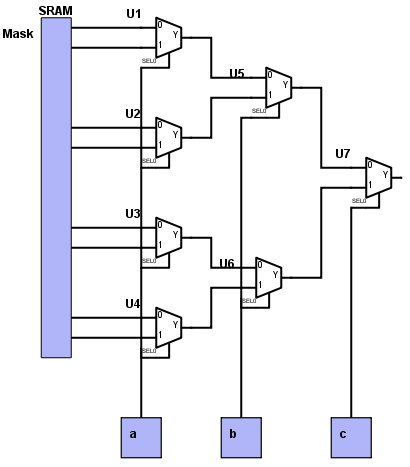
\includegraphics[height=.75\textheight,left]{lutMux.jpg}
\caption{$3$ stages of $2x1$ MUX}
\end{figure}

\column{.5\textwidth}
\begin{itemize}
\item It is a \alert{table} that ditermines what the output is for any given input
\item A \alert{state-less} interconnection of any number of gates \\(no feedback loops)
\item Implemented \emph{multiplexing} a combination of SRAM bits 
\end{itemize}


\end{columns}

\end{frame}
%------------------------------------------------

\begin{frame}
\frametitle{FPGAs Structure}
\framesubtitle{LUT Example}

$$y = ( a + b ) \cdot c $$

\begin{columns}[c]


\column{.4\textwidth}

\begin{table}
\centering
\begin{tabular}{c|c}
a b c & y \\
\hline
0 0 0 & 0\\
0 0 1 & 0\\
0 1 0 & 0\\
0 1 1 & 0\\
1 0 0 & 0\\
1 0 1 & 1\\
1 1 0 & 0\\
1 1 1 & 1\\

\end{tabular}
\end{table}

\column{.6\textwidth}
\centering
\begin{figure}
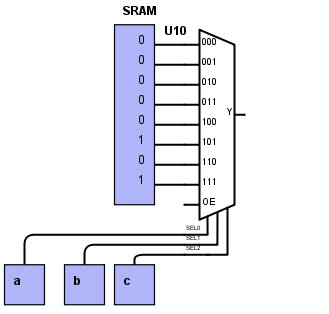
\includegraphics[width=.9\linewidth,left]{lutExplan.jpg}
\caption{$y = ( a + b ) \cdot c $ }
\end{figure}

\end{columns}
\end{frame}
%------------------------------------------------
\begin{frame}
\subsection{Basic Logic Element}
\frametitle{FPGAs structure}
\framesubtitle{BLE}

\begin{figure}
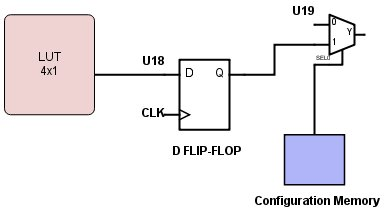
\includegraphics[width=.9\linewidth,left]{lutBle.jpg}
\caption{Basic Logic Element}
\end{figure}

\end{frame}
%------------------------------------------------
\begin{frame}
\subsection{Overview}
\frametitle{FPGAs structure}
\framesubtitle{Overview}

\begin{figure}
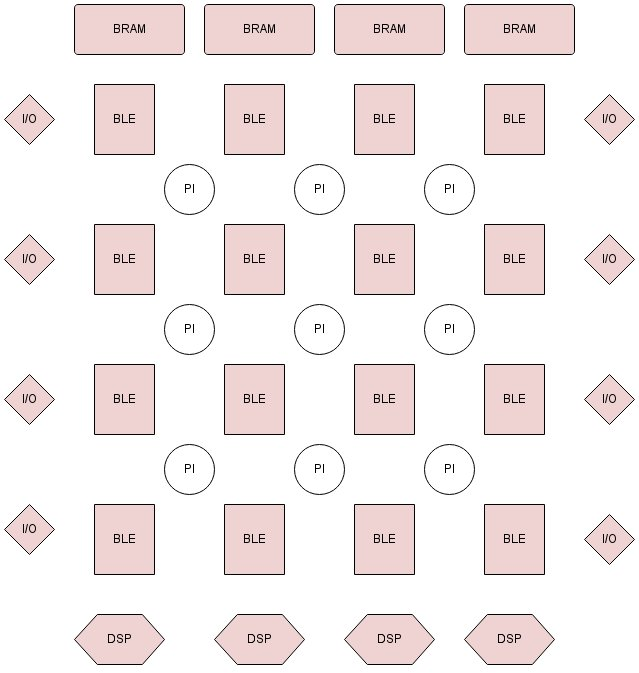
\includegraphics[width=.58\linewidth,center]{full.jpg}
\caption{FPGAs Complete Overview}
\end{figure}

\end{frame}


%------------------------------------------------
%------------------------------------------------
%------------------------------------------------
%------------------------------------------------
%------------------------------------------------
%------------------------------------------------
%------------------------------------------------

\iffalse

\begin{frame}
\frametitle{Parallel Architectures}
\begin{columns}[c]

\column{.8\textwidth}
\linespread{0.5}
\begin{block}{Shared Memory}
\begin{enumerate}
\item {\fontsize{8}{6}\selectfont Processors share the same physical memory}
\item {\fontsize{8}{6}\selectfont Local cache memory hierarchy}
\item {\fontsize{8}{6}\selectfont Connection via memory bus}
\end{enumerate}
\end{block}

\begin{block}{Distributed Memory}
\begin{enumerate}
\item {\fontsize{8}{6}\selectfont Every processor has its own memory hierarcy}
\item {\fontsize{8}{6}\selectfont Processor communication via interconnection network}
\end{enumerate}
\end{block}

\begin{block}{Hybrid Architectures}
Dominant architecture for modern supercomputers.
\end{block}

\column{.3\textwidth}
\begin{figure}
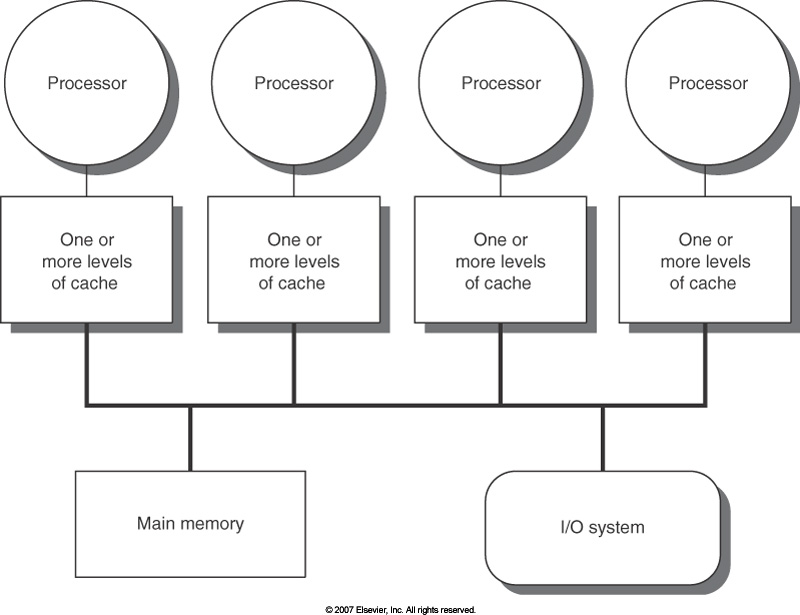
\includegraphics[width=\linewidth,right]{shared_mem.jpg}
\end{figure}

\begin{figure}
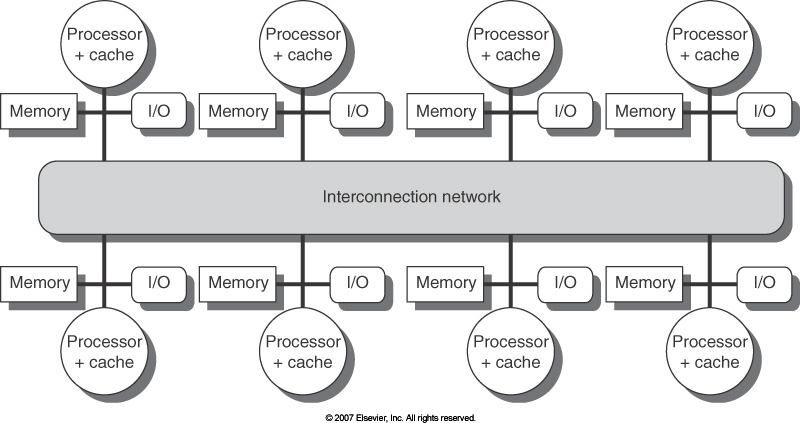
\includegraphics[width=\linewidth,right]{distributed_mem.jpg}
\end{figure}

\begin{figure}
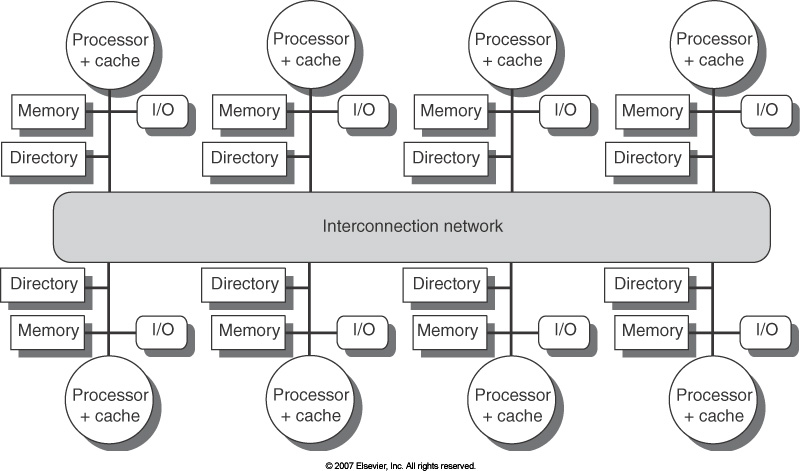
\includegraphics[width=\linewidth,right]{hybrid_mem.jpg}
\end{figure}

\end{columns}

\end{frame}


\fi
%------------------------------------------------


\end{document} 
%----------------------------------------------------------------------------------------
